\documentclass{beamer}

\usepackage{beamerthemesplit}
\usepackage{graphicx}
\usepackage{color, natbib, hyperref}
\usepackage{bibentry}
\usepackage[export]{adjustbox}% http://ctan.org/pkg/adjustbox
\usepackage{multicol}
\usepackage{tikz}
\usetikzlibrary{calc}
\usepackage{array}
\newcolumntype{L}{>{\centering\arraybackslash}m{2.5cm}}


\nobibliography*

% define colors
\definecolor{jblue}  {RGB}{20,50,100}
\definecolor{ngreen} {RGB}{98,158,31}

%theme

\usetheme{boxes} 
%\usecolortheme{seahorse} 
\setbeamertemplate{items}[default] 
%\setbeamercovered{transparent}
\setbeamertemplate{blocks}[rounded]
\setbeamertemplate{navigation symbols}{} 
% set the basic colors
\setbeamercolor{palette primary}   {fg=black,bg=white}
\setbeamercolor{palette secondary} {fg=black,bg=white}
\setbeamercolor{palette tertiary}  {bg=jblue,fg=white}
\setbeamercolor{palette quaternary}{fg=black,bg=white}
\setbeamercolor{structure}{fg=jblue}
\setbeamercolor{titlelike}{bg=jblue,fg=white}
\setbeamercolor{frametitle}{bg=jblue!10,fg=jblue}
\setbeamercolor{cboxb}{fg=black,bg=jblue}
\setbeamercolor{cboxr}{fg=black,bg=red}

% reduce space before/after equations
\expandafter\def\expandafter\normalsize\expandafter{%
    \normalsize
    \setlength\abovedisplayskip{1pt}
    \setlength\belowdisplayskip{1pt}
    \setlength\abovedisplayshortskip{1pt}
    \setlength\belowdisplayshortskip{1pt}
}

% set colors for itemize/enumerate
\setbeamercolor{item}{fg=ngreen}
\setbeamercolor{item projected}{fg=white,bg=ngreen}

% set colors for blocks
\setbeamercolor{block title}{fg=ngreen,bg=white}
\setbeamercolor{block body}{fg=black,bg=jblue!10}

% set colors for alerted blocks (blocks with frame)
\setbeamercolor{block alerted title}{fg=white,bg=jblue}
\setbeamercolor{block alerted body}{fg=black,bg=jblue!10}
\setbeamercolor{block alerted title}{fg=white,bg=dblue!70} % Colors of the highlighted block titles
\setbeamercolor{block alerted body}{fg=black,bg=dblue!10} % Colors of the body of highlighted blocks

% set the fonts
\usefonttheme{professionalfonts}

\setbeamerfont{section in head/foot}{series=\bfseries}
\setbeamerfont{block title}{series=\bfseries}
\setbeamerfont{block alerted title}{series=\bfseries}
\setbeamerfont{frametitle}{series=\bfseries}
\setbeamerfont{frametitle}{size=\Large}
\setbeamerfont{block body}{series=\mdseries}
\setbeamerfont{caption}{series=\mdseries}
\setbeamerfont{headline}{series=\mdseries}


% set some beamer theme options
\setbeamertemplate{title page}[default][colsep=-4bp,rounded=true]
\setbeamertemplate{sections/subsections in toc}[square]
\setbeamertemplate{items}[circle]
\setbeamertemplate{blocks}[width=0.0]
\beamertemplatenavigationsymbolsempty

% Custom colors
\usepackage{color}
%\definecolor{deepblue}{rgb}{0,0,0.5}
%\definecolor{deepred}{rgb}{0.6,0,0}
%\definecolor{deepgreen}{rgb}{0,0.5,0}
\definecolor{Code}{rgb}{0,0,0}
\definecolor{Decorators}{rgb}{0.5,0.5,0.5}
\definecolor{Numbers}{rgb}{0.5,0,0}
\definecolor{MatchingBrackets}{rgb}{0.25,0.5,0.5}
\definecolor{Strings}{rgb}{0.75,0,0}
\definecolor{self}{rgb}{0,0,0}
\definecolor{Keywords}{rgb}{0,0.63,0}
\definecolor{Comments}{rgb}{0,0.63,1}
\definecolor{Backquotes}{rgb}{0,0,0}
\definecolor{Classname}{rgb}{0,0,0}
\definecolor{FunctionName}{rgb}{0,0,0}
\definecolor{Operators}{rgb}{0,0,0}

% Default fixed font does not support bold face
\usepackage[utf8]{inputenc}
\DeclareFixedFont{\ttb}{T1}{txtt}{bx}{n}{12} % for bold
\DeclareFixedFont{\ttm}{T1}{txtt}{m}{n}{12}  % for normal

% Python style for highlighting
\usepackage{listings}
\newcommand\pythonstyle{\lstset{
language=Python,
%numbers=left,
%numberstyle=\footnotesize,
%numbersep=1em,
%xleftmargin=1em,
framextopmargin=0em,
framexbottommargin=0em,
showspaces=false,
showtabs=false,
showstringspaces=false,
frame=l,
tabsize=4,
% Basic
basicstyle=\ttfamily\scriptsize,
otherkeywords={self},             % Add keywords here
keywordstyle={\color{Keywords}\bfseries},
% Comments
commentstyle=\color{Comments}\slshape,
%% Strings
stringstyle=\color{Strings},
morecomment=[s][\color{Strings}]{"""}{"""},
morecomment=[s][\color{Strings}]{'''}{'''},
% keywords
morekeywords={import,from,class,def,for,while,if,is,in,elif,else,not,and,or,print,break,continue,return,True,False,None,access,as,,del,except,exec,finally,global,import,lambda,pass,print,raise,try,assert},
keywordstyle={\color{Keywords}\bfseries},
% additional keywords
morekeywords={[2]@invariant,pylab,numpy,np,scipy},
keywordstyle={[2]\color{Decorators}\slshape},
emph={self},
emphstyle={\color{self}\slshape},
frame=tb,                         % Any extra options here
showstringspaces=false            % 
}}

% Python environment
\lstnewenvironment{python}[1][]
{
\pythonstyle
\lstset{#1}
}
{}

% Python for external files
\newcommand\pythonexternal[2][]{{
\pythonstyle
\lstinputlisting[#1]{#2}}}

% Python for inline
\newcommand\pythoninline[1]{{\pythonstyle\lstinline!#1!}}



% Math macros
\newcommand{\cD}{{\mathcal D}}
\newcommand{\cF}{{\mathcal F}}
\newcommand{\todo}[1]{{\color{red}{TO DO: \sc #1}}}

\newcommand{\reals}{\mathbb{R}}
\newcommand{\integers}{\mathbb{Z}}
\newcommand{\naturals}{\mathbb{N}}
\newcommand{\rationals}{\mathbb{Q}}

\newcommand{\ind}[1]{1_{#1}} % Indicator function
\newcommand{\pr}{\mathbb{P}} % Generic probability
\newcommand{\ex}{\mathbb{E}} % Generic expectation
\newcommand{\var}{\textrm{Var}}
\newcommand{\cov}{\textrm{Cov}}

\newcommand{\normal}{N} % for normal distribution (can probably skip this)
\newcommand{\eps}{\varepsilon}
\newcommand\independent{\protect\mathpalette{\protect\independenT}{\perp}}
\def\independenT#1#2{\mathrel{\rlap{$#1#2$}\mkern2mu{#1#2}}}

\newcommand{\convd}{\stackrel{d}{\longrightarrow}} % convergence in distribution/law/measure
\newcommand{\convp}{\stackrel{P}{\longrightarrow}} % convergence in probability
\newcommand{\convas}{\stackrel{\textrm{a.s.}}{\longrightarrow}} % convergence almost surely

\newcommand{\eqd}{\stackrel{d}{=}} % equal in distribution/law/measure
\newcommand{\argmax}{\arg\!\max}
\newcommand{\argmin}{\arg\!\min}

% Making a DAG
\usepackage{tkz-graph}  
\usetikzlibrary{calc}
\usetikzlibrary{shapes.geometric}
\usetikzlibrary{positioning}
\tikzstyle{VertexStyle} = [shape            = rectangle,
                               minimum width    = 6ex,%
                               draw]
 \tikzstyle{EdgeStyle}   = [->,>=stealth']      

% Define block styles
\tikzstyle{f} = [rectangle, draw, fill=blue!20, 
    text width=3em, text badly centered, node distance=1.75cm]
\tikzstyle{message} = [rectangle, draw, fill=green!20, 
    text width=3em, text centered]
\tikzstyle{io} = [draw, circle,fill=red!20, node distance=2cm,
    minimum height=2em]
\tikzstyle{line} = [draw, -latex']


\mode<presentation>

\title[permute]{From Paper to Program: Challenges of Implementing Permutation Tests}
\author{\Large Kellie Ottoboni \\
\small with Philip~B. Stark}
\institute[]{Department of Statistics, UC Berkeley\\Berkeley Institute for Data Science}
\date{June 12, 2018\\\small ISNPS, Salerno}

\begin{document}

\frame{
\titlepage
\vfill
\begin{columns}[T]
\begin{column}{.5\textwidth}
\begin{center}
\vspace{25pt}

\includegraphics[width=\textwidth]{fig/logo/dept1.pdf}
\end{center}
\end{column}
\begin{column}{.3\textwidth}
\end{column}
\begin{column}{.3\textwidth}
\begin{center}

\includegraphics[width=0.9\textwidth]{fig/logo/BIDS.png}
\end{center}
\end{column}
\end{columns}
}


%
%\frame{
%\frametitle{Collaborators}
%\begin{figure}[htbp]
%\begin{center}
%\includegraphics[width = 0.3\textwidth, valign=t]{fig/github/jarrodmillman} 
%\includegraphics[width = 0.3\textwidth, valign=t]{fig/github/pbstark} 
%\includegraphics[width = 0.3\textwidth, valign=t]{fig/github/stefanv} 
%\end{center}
%\end{figure}
%
%}


%\AtBeginSection[]
%{
%   \begin{frame}
%       \frametitle{Outline}
%       \tableofcontents%[currentsection]
%   \end{frame}
%}


\section[Introduction]{Introduction}



\usebackgroundtemplate{%             declare it
\tikz[overlay,remember picture] \node[opacity=0.3, at=(current page.center)] {
   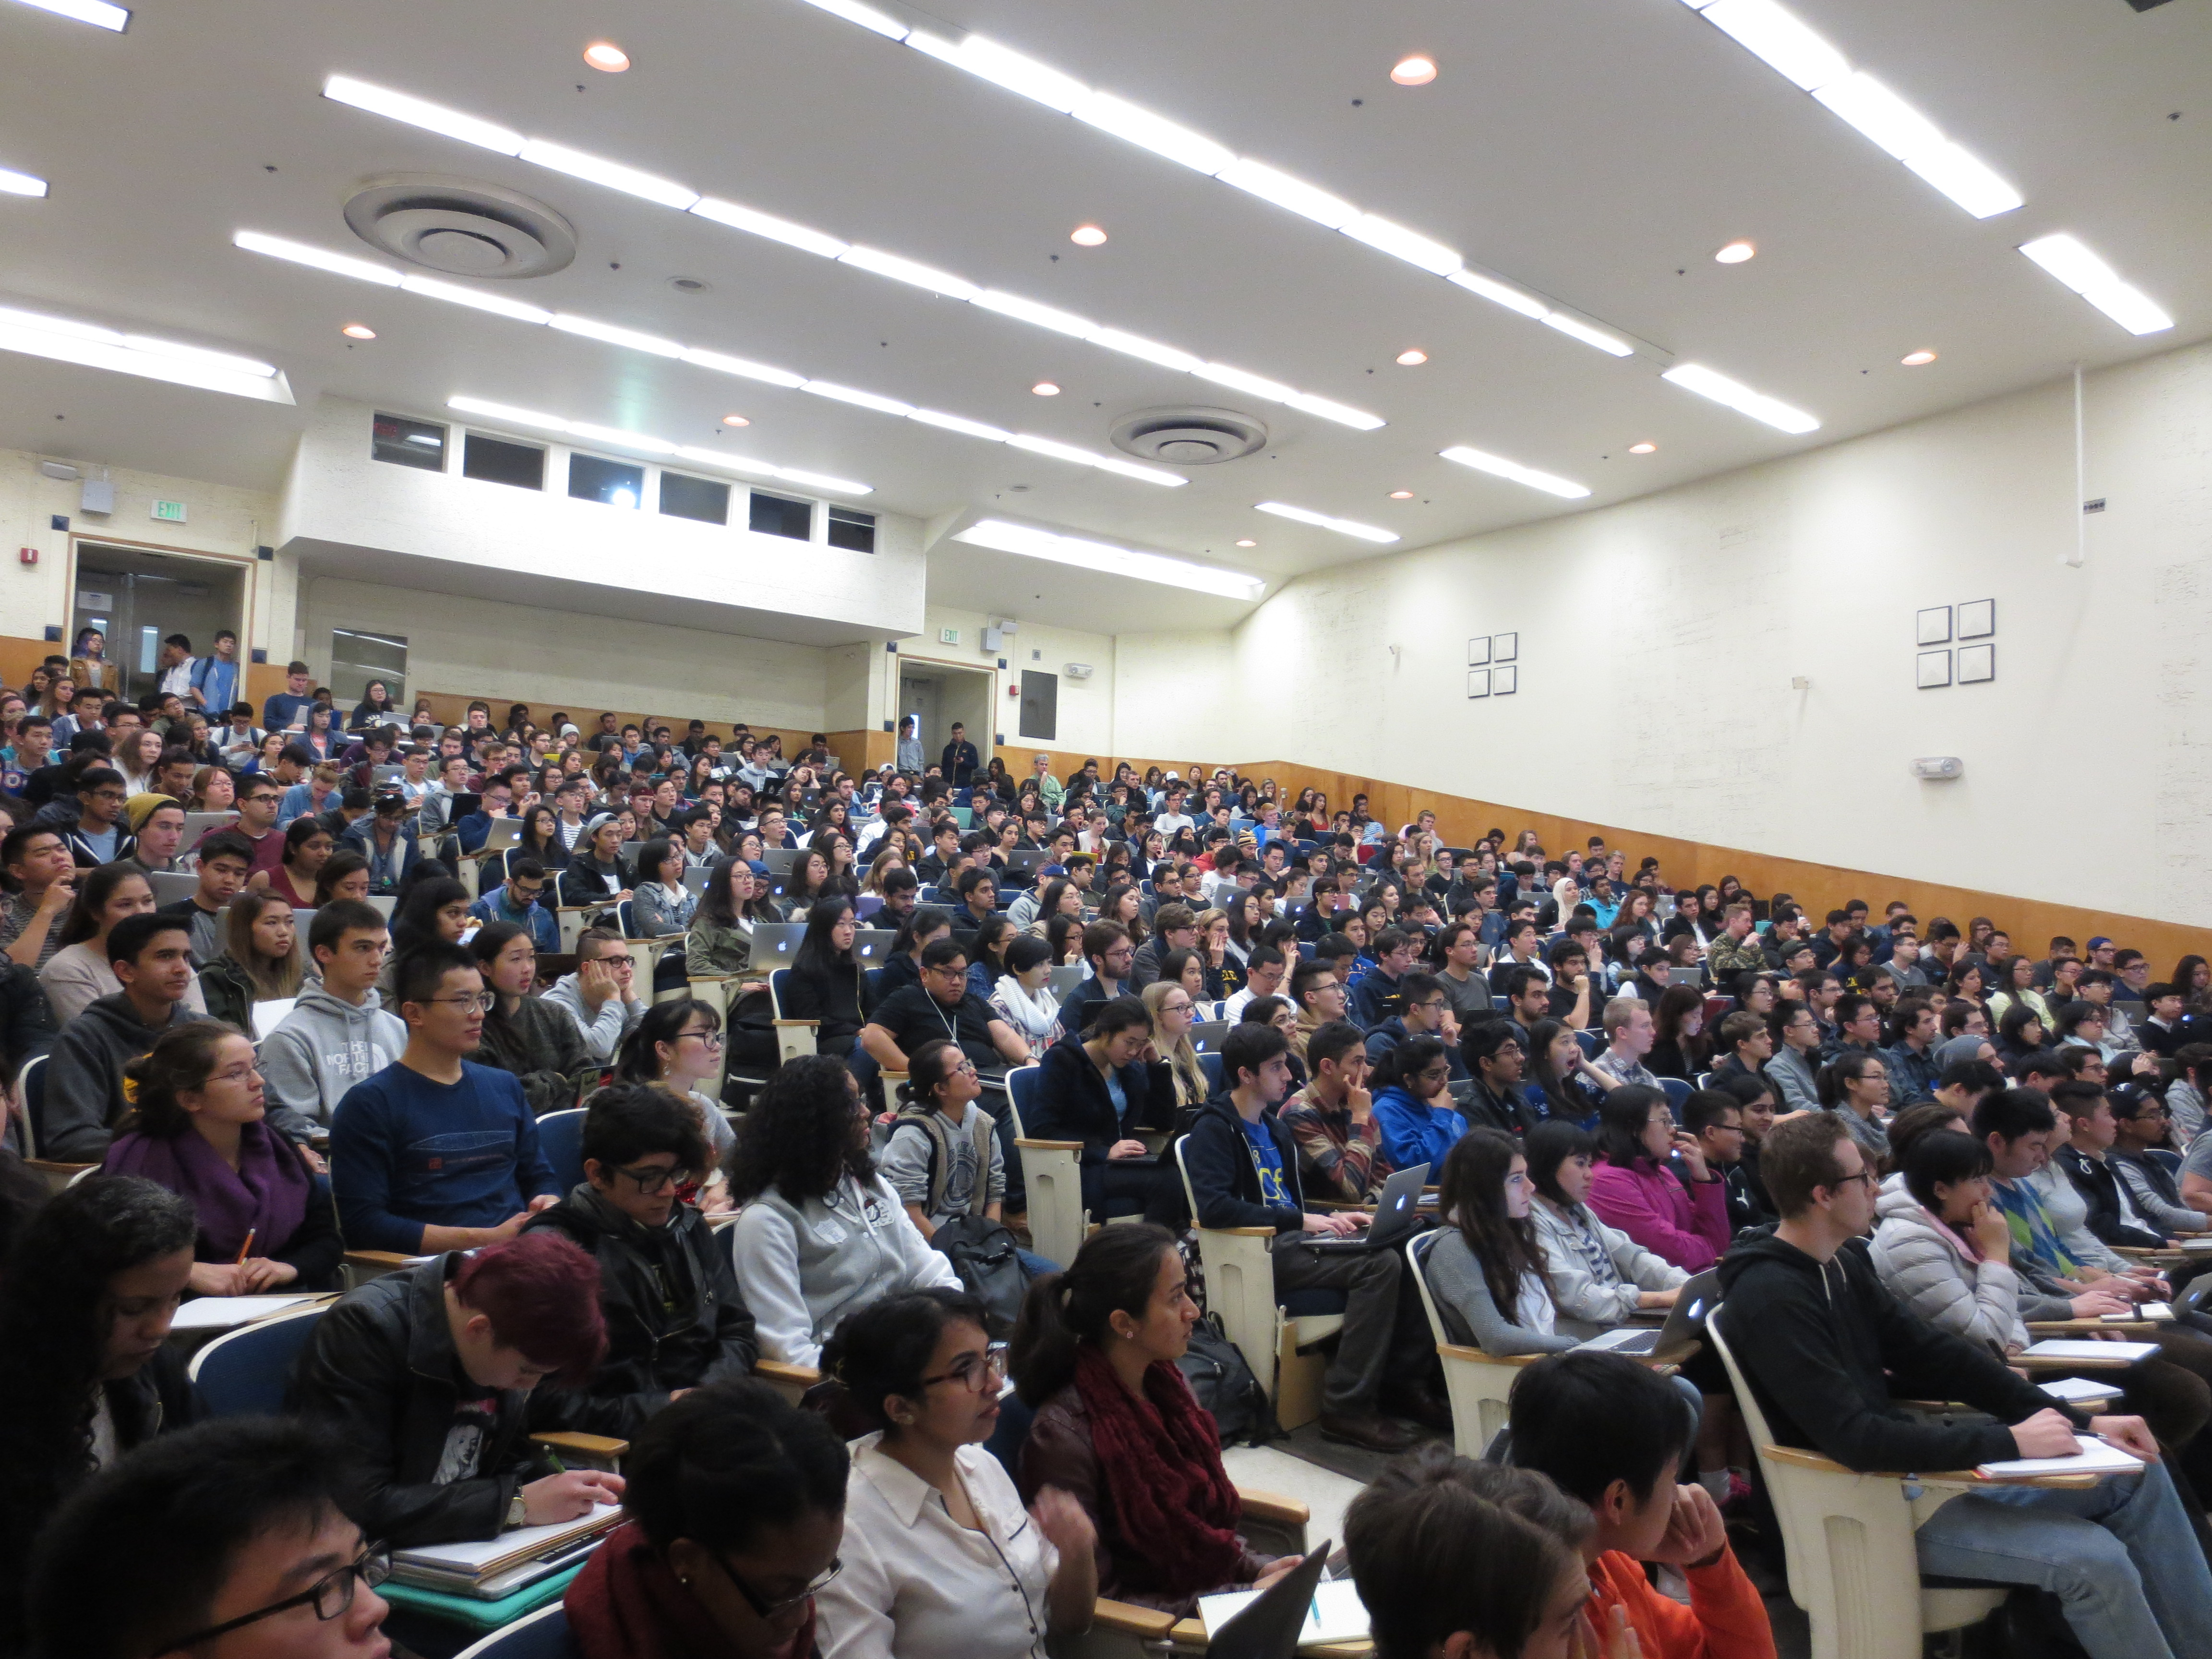
\includegraphics[height=\paperheight,width=\paperwidth]{fig/DS8.jpg}};
}


\frame{
\begin{center}
\Huge
Teaching Introductory Statistics
\end{center}
}

\usebackgroundtemplate{ }    %% undeclare it



\frame{
\frametitle{Introductory Statistics}

% When I meet new people and tell them I'm a statistician, the most common response I get is
% wow, good for you, I took one statistics class and I hated it/was terrible at it
\Large
\begin{columns}[T]
\begin{column}{.5\textwidth}
\begin{center}

Important concepts
\vspace{10pt}

\begin{itemize}
\item Sampling distributions 
\item $p$-values
\item Confidence intervals
\end{itemize}

\end{center}
\end{column}

\pause
\begin{column}{.5\textwidth}
\begin{center}

Barriers to learning
\vspace{10pt}
\begin{itemize}
\item Z tests, t tests
\item Assumptions
\item Formulas
\end{itemize}

\end{center}
\end{column}

\end{columns}





%Students leave intro stats thinking that statistics is pedantic and all about memorizing formulas.
%They think that $t$ tests are the only way to analyze data!

}


\frame{
\frametitle{What if we could teach the concepts without the particular details?}

\begin{columns}

\Large

\begin{column}{.5\textwidth}
Tools:

\begin{enumerate}
\item Resampling methods
\item Computers
\end{enumerate}

\end{column}
\begin{column}{.5\textwidth}
\begin{center}
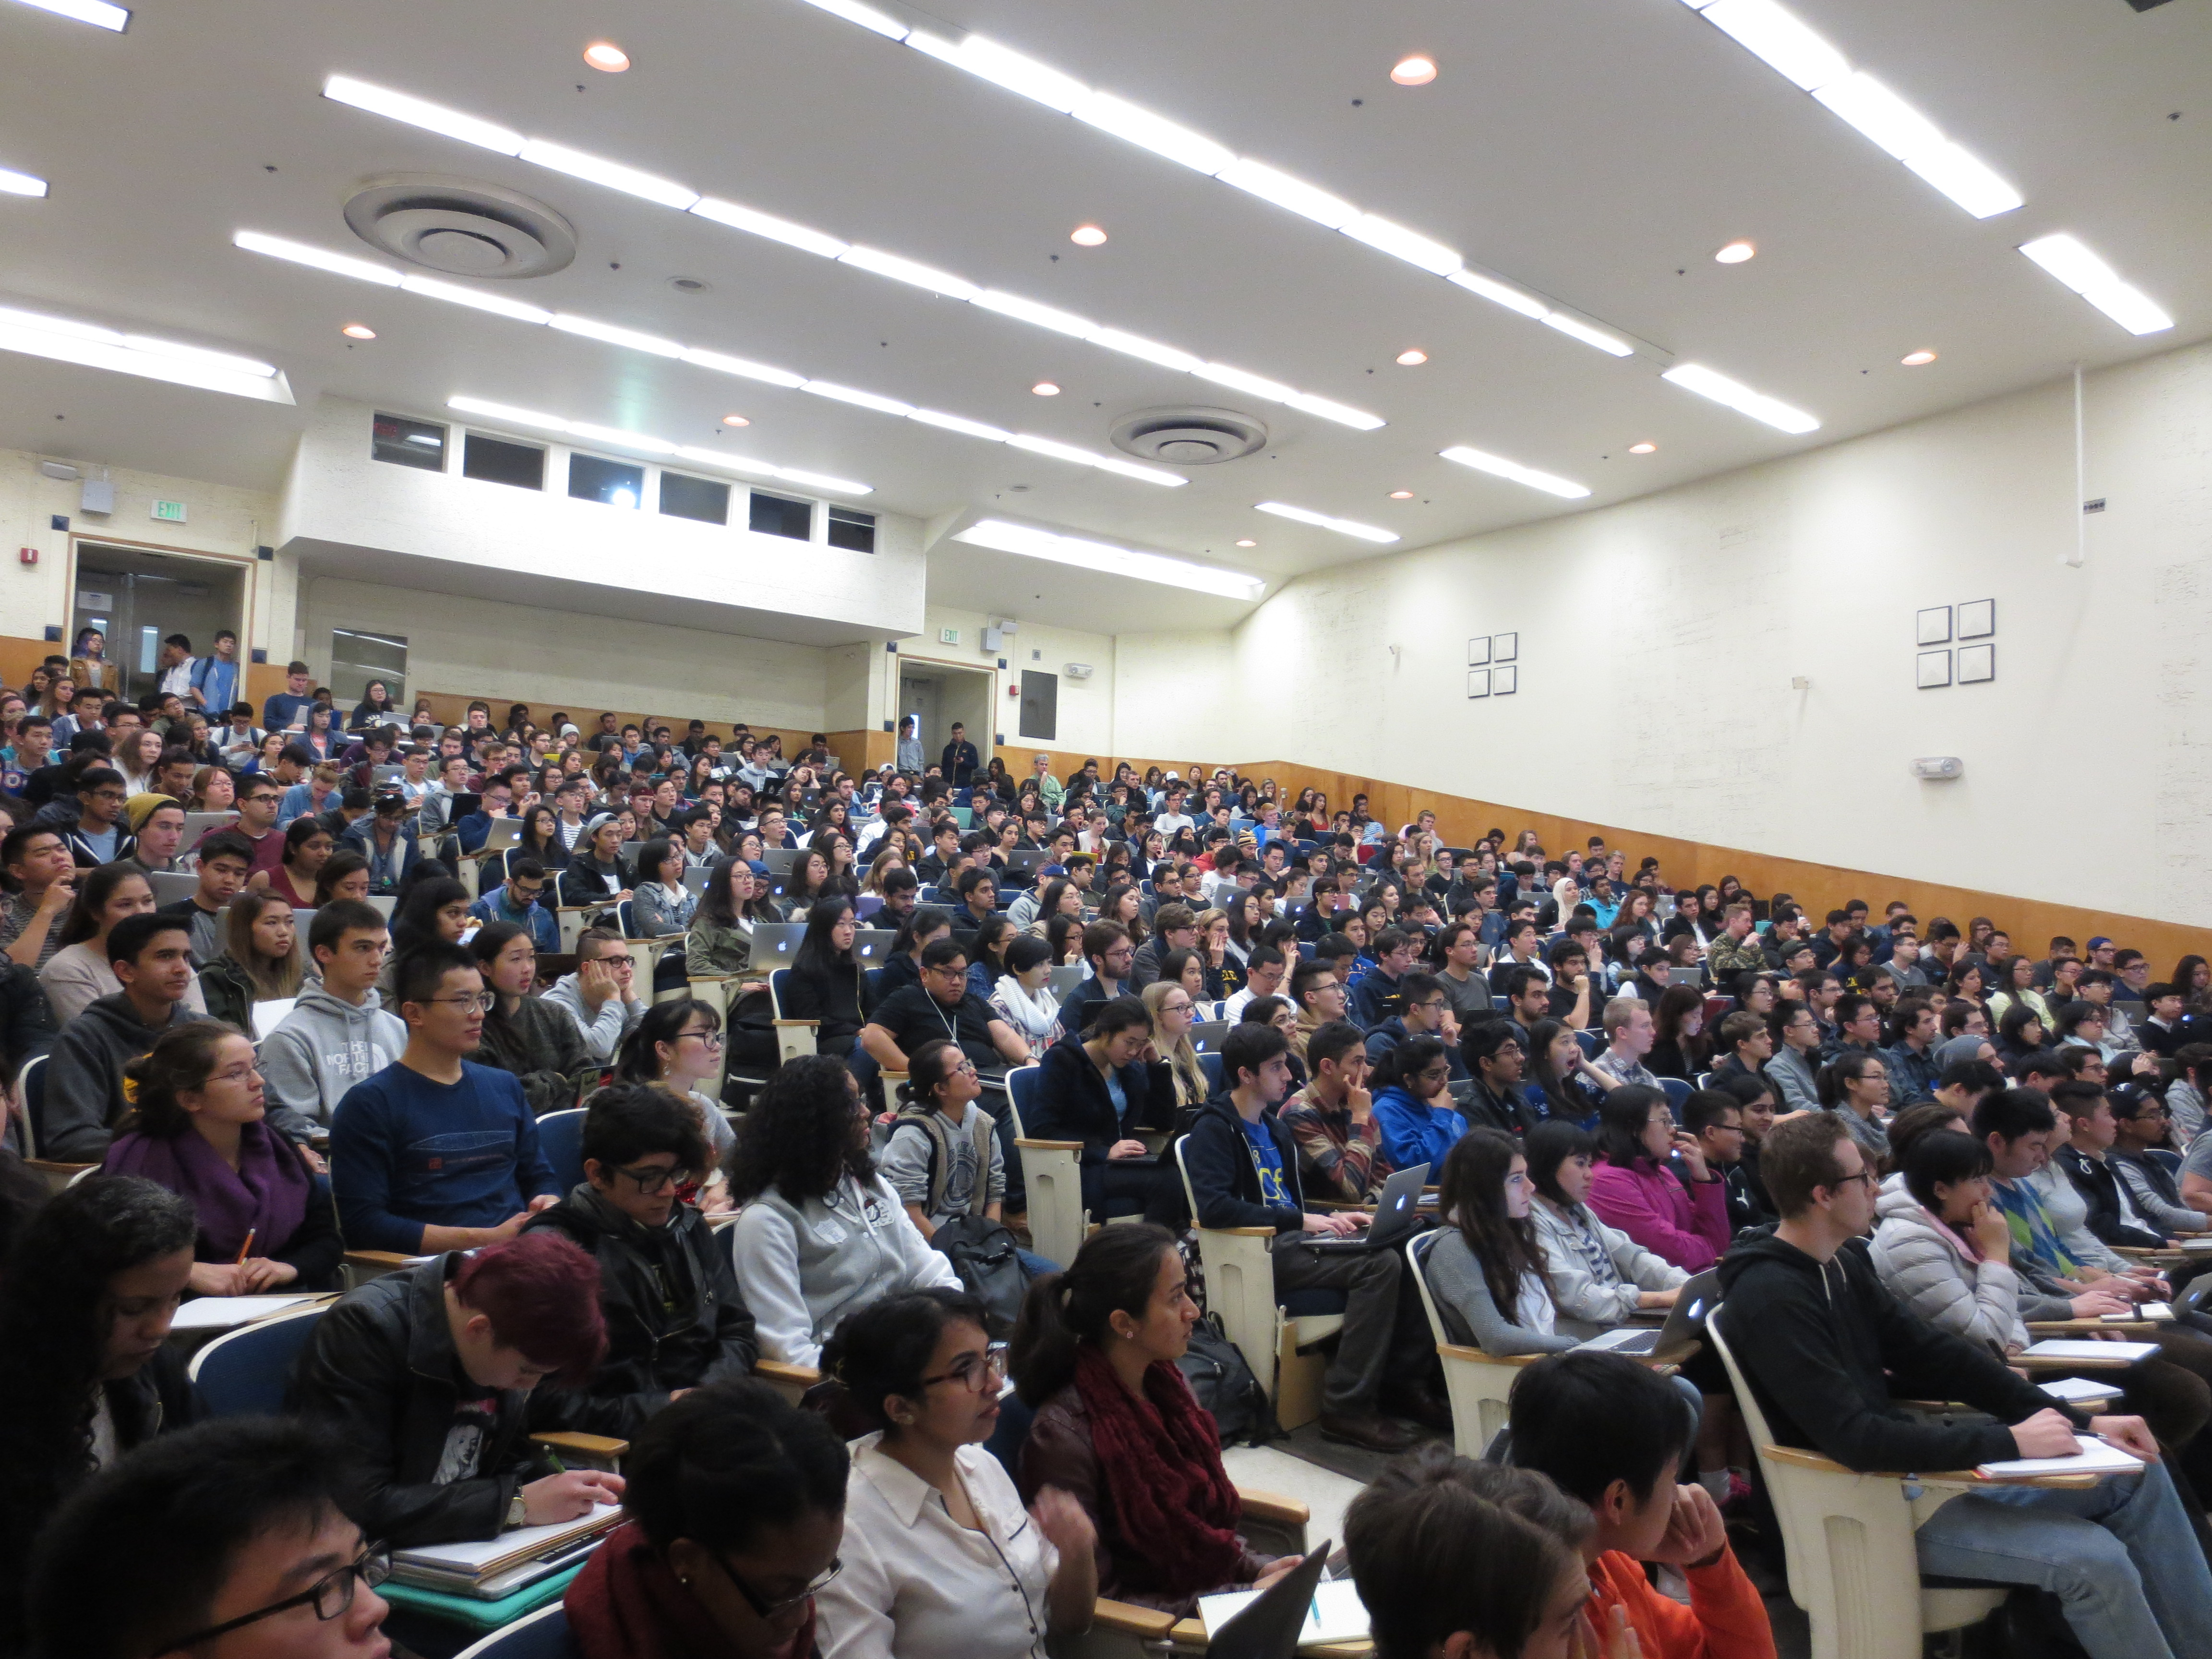
\includegraphics[width=0.9\textwidth]{fig/DS8.jpg} \\
Data Science 8 \\ UC Berkeley
\end{center}
\end{column}
\end{columns}
}


\frame{
\frametitle{Permutation tests clarify concepts.}

\Large
\begin{itemize}
\item General: it's a procedure, not a formula
\item Discrete: counting instead of integration
\item Design-based: assumptions come from the data collection
\end{itemize}


\vfill
\small \textit{Hesterberg (2015)}

}




\frame{
\frametitle{Python is gaining popularity for data analysis.}
\Large

\begin{itemize}
\item General purpose language, ``batteries included''
\item Libraries for a variety of scientific applications
\end{itemize}

\begin{figure}[htbp]
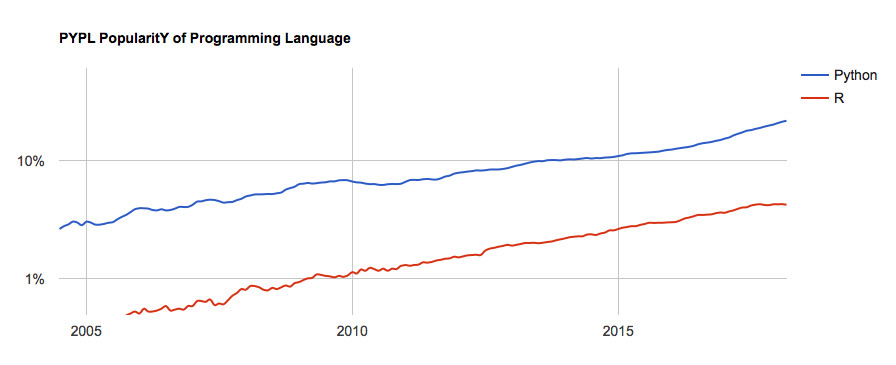
\includegraphics[scale=0.3]{fig/pypl}
\end{figure}


}



%\frame{
%\frametitle{Python for teaching Statistics}
%\begin{center}
%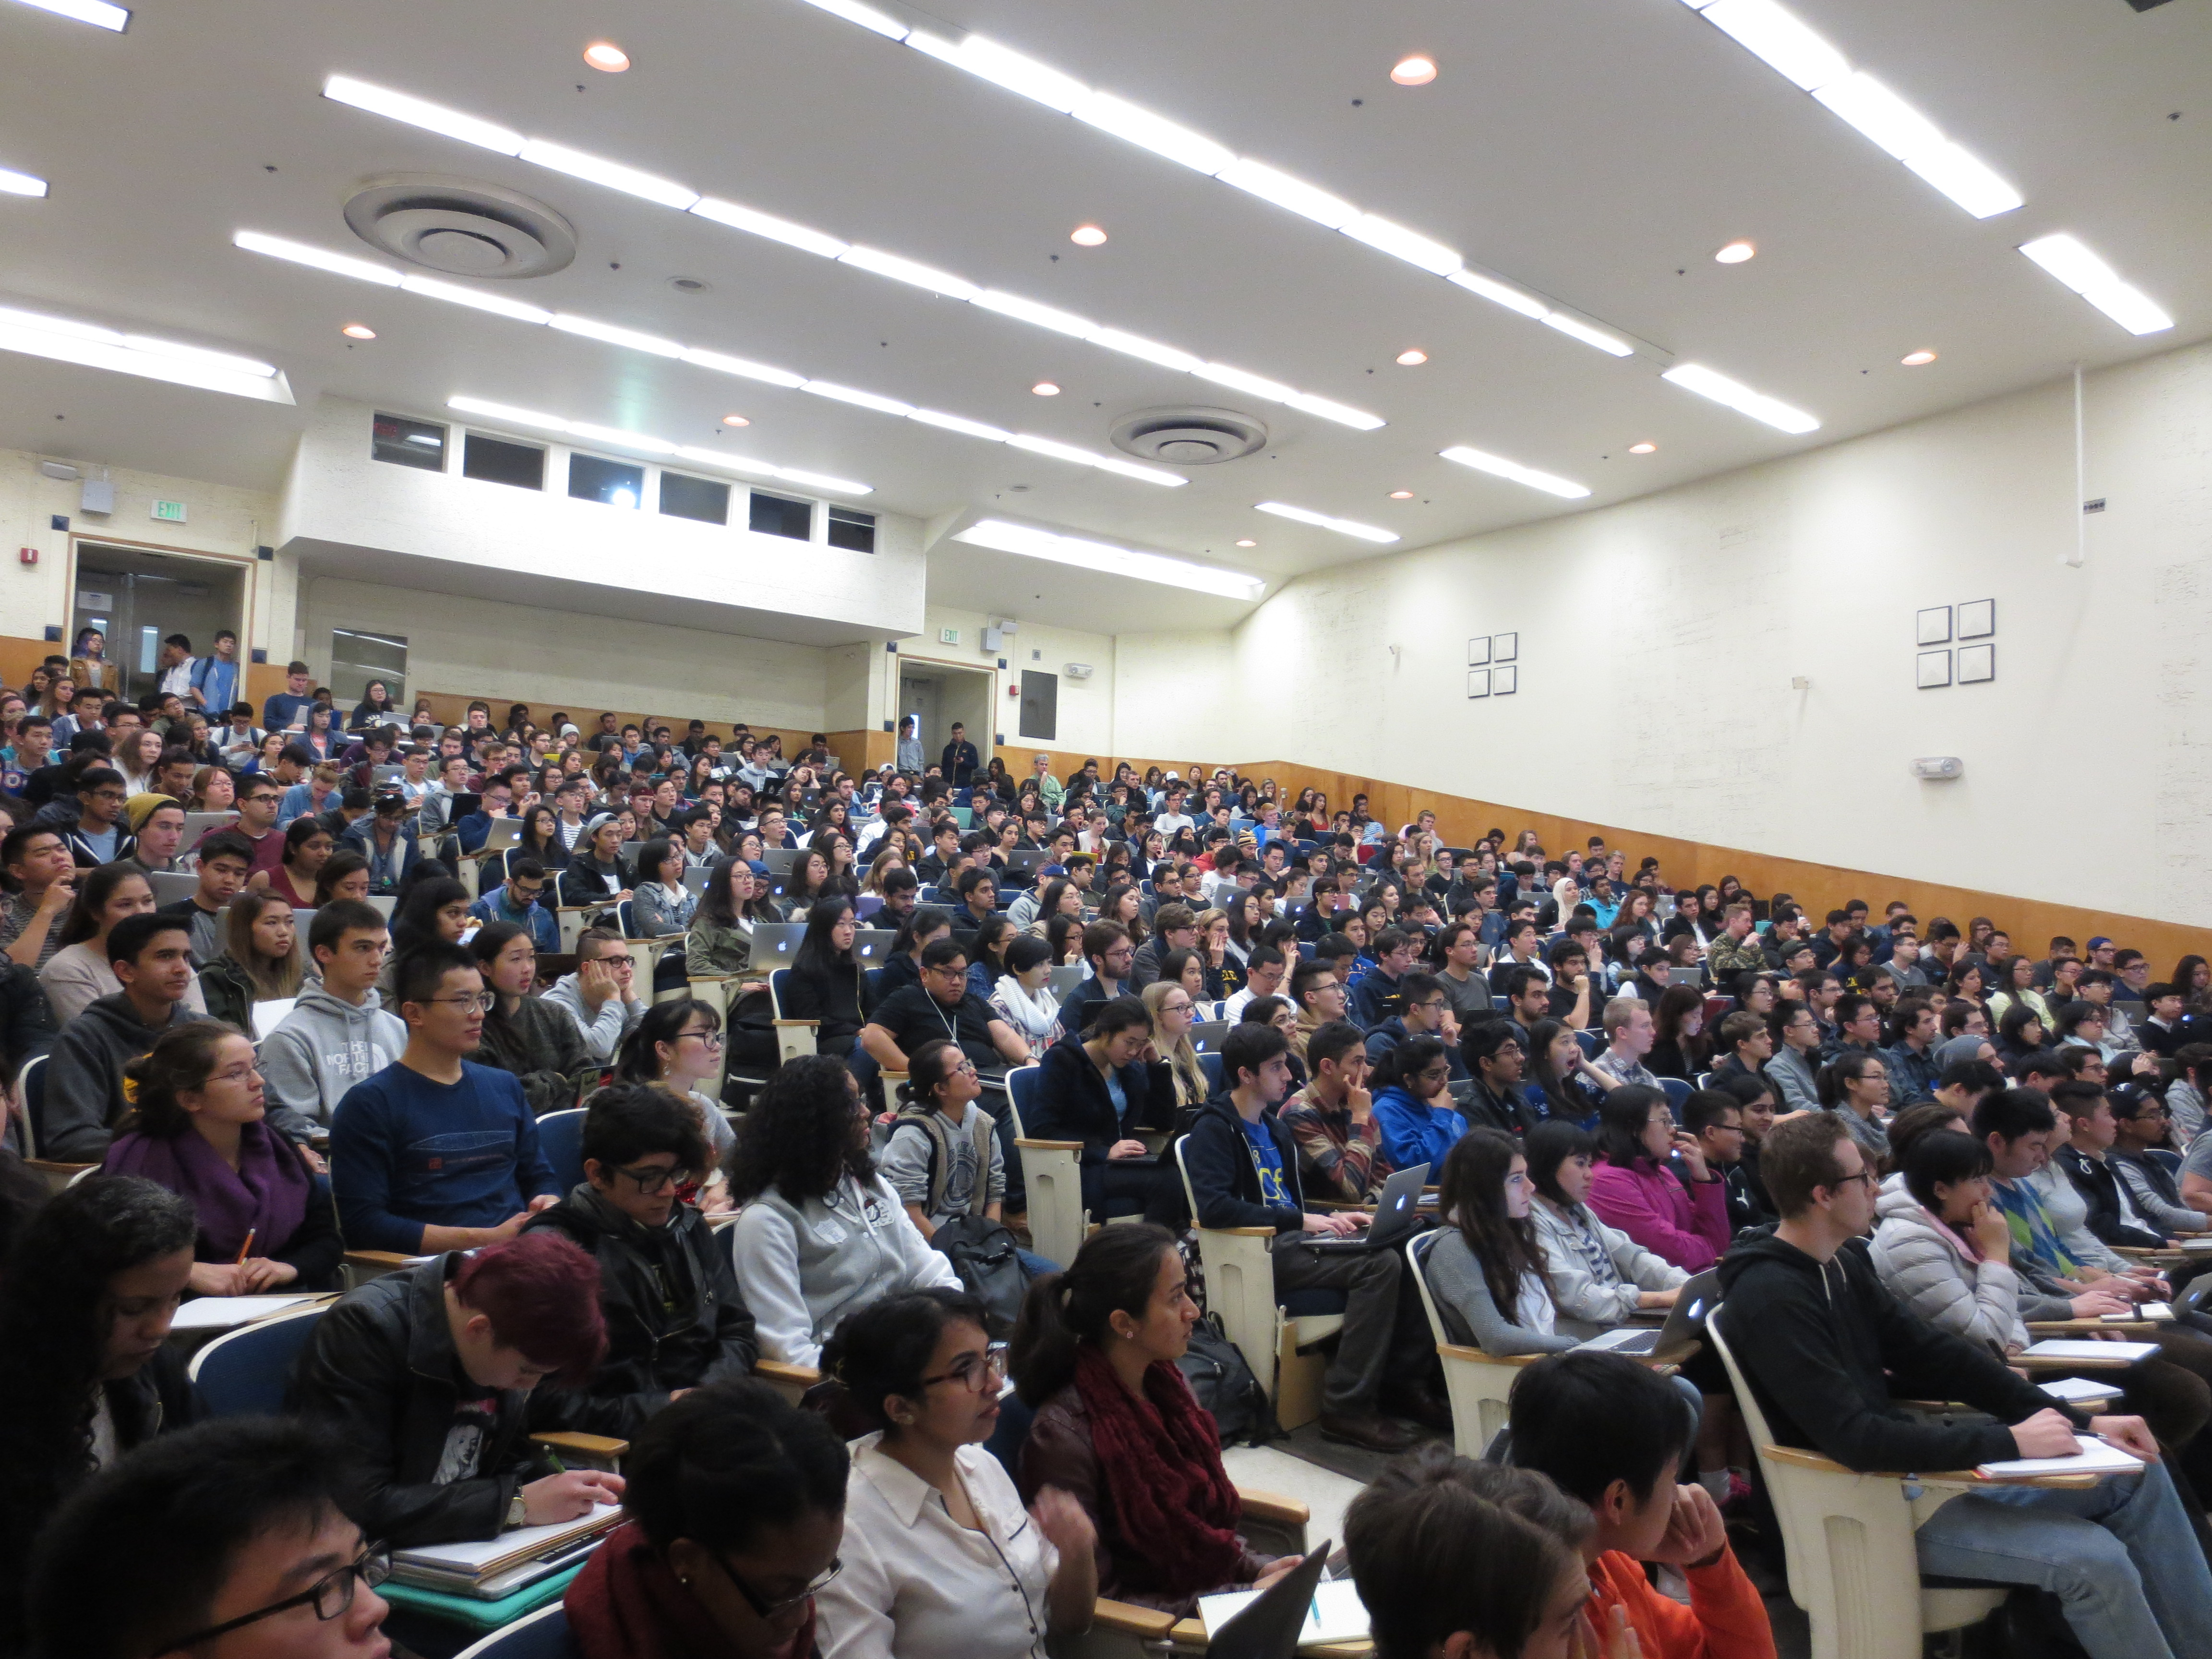
\includegraphics[width=0.9\textwidth]{fig/DS8.jpg} \\
%Data Science 8 at UC Berkeley
%\end{center}
%}



\section[The book]{The book}

\usebackgroundtemplate{%             declare it
\tikz[overlay,remember picture] \node[opacity=0.3, at=(current page.center)] {
   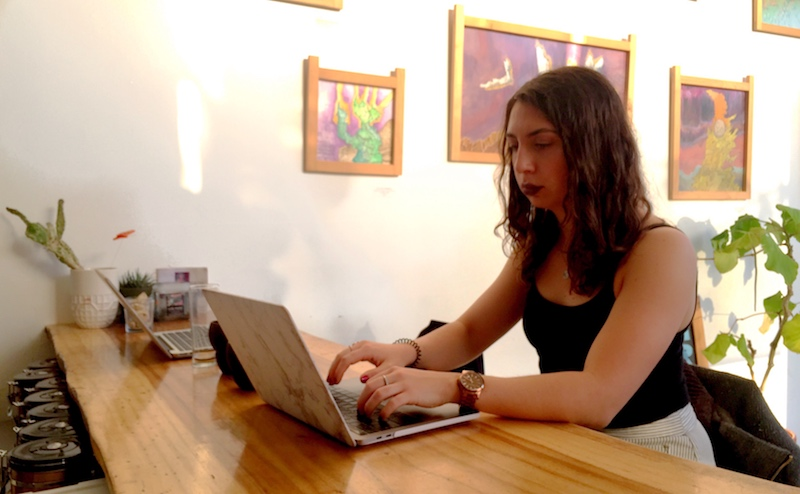
\includegraphics[height=\paperheight,width=1.2\paperwidth]{fig/working.jpg}};
}


\frame{
\begin{center}
\Huge
The book
\end{center}
}

\usebackgroundtemplate{ }    %% undeclare it



\frame{
\frametitle{A companion to Pesarin and Salmaso (2010)}

\begin{columns}[T]
\begin{column}{.4\textwidth}
\begin{center}
%\vspace{25pt}

\includegraphics[width=0.9\textwidth]{fig/pesarinsalmaso.jpg}
\end{center}
\end{column}
\begin{column}{.6\textwidth}

\begin{itemize}
\item Target audience: late undergraduate to early PhD or domain researchers with some statistics background
\item Conceptual: how to determine an appropriate permutation test
\item Carefully consider experimental design and assumptions
\item Introduce concepts about causal inference
\end{itemize}

\end{column}
\end{columns}


}


\frame{
\frametitle{Three chapters}
\Large
\begin{enumerate}
\setlength\itemsep{20pt}
\item Components of a permutation test \\
\normalsize \qquad The null invariance and the test statistic
\item \Large From experiments to observational studies \\
\normalsize \qquad Randomization, confounding, the ``implied experiment''
\item \Large Computation for permutation tests \\
\normalsize \qquad Sampling algorithms and pseudorandom numbers
\end{enumerate}
}



\frame{
\frametitle{The book will be open-source online...}
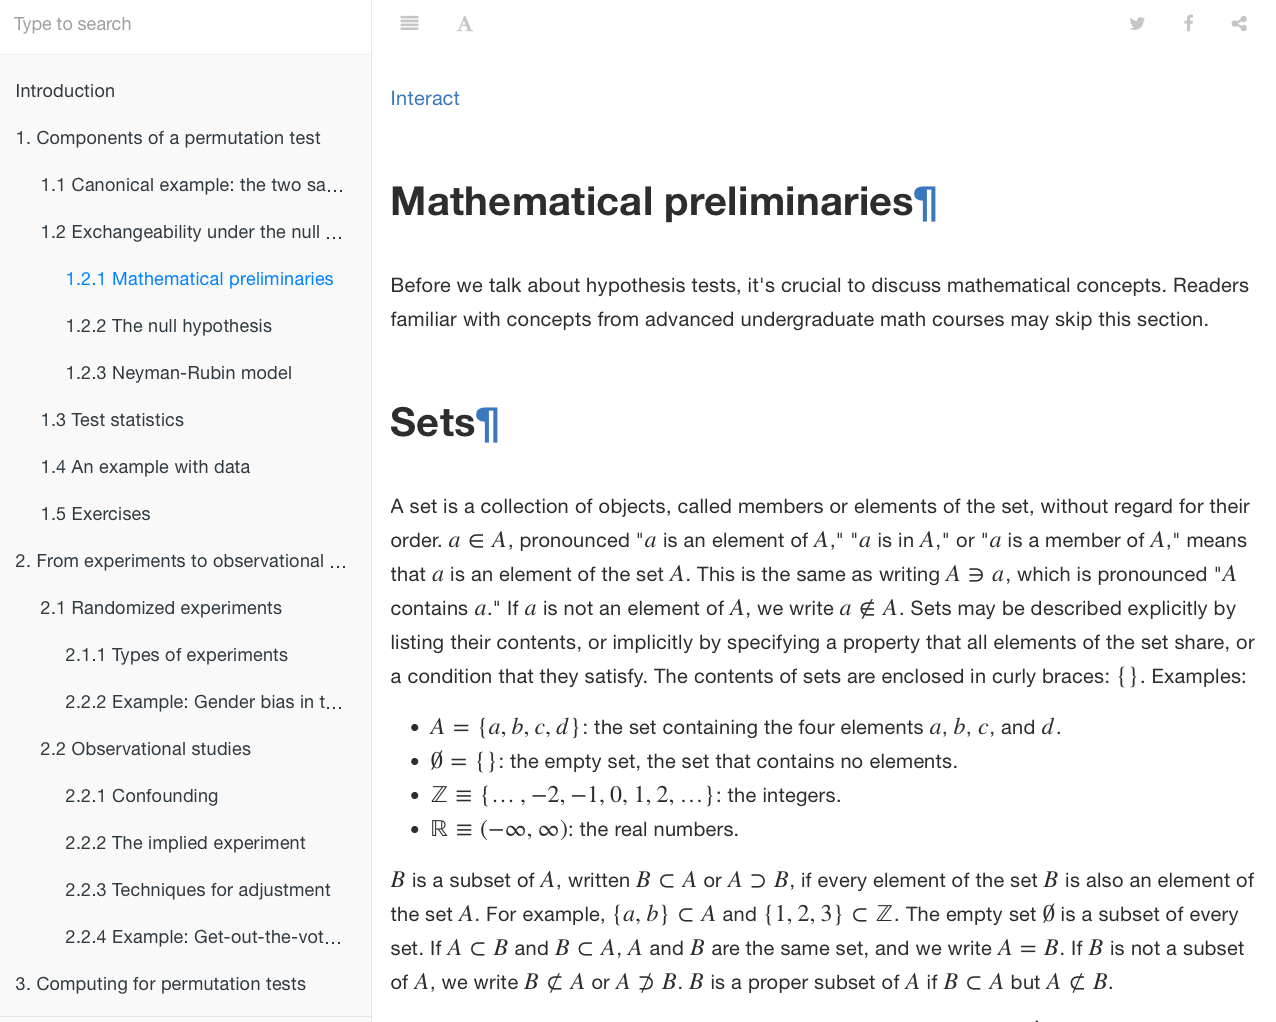
\includegraphics[height=1.3\paperheight]{fig/gitbook.png}
}

\frame{
\frametitle{with interactive Python code.}

\begin{center}
\begin{tikzpicture}
  \node (img1) {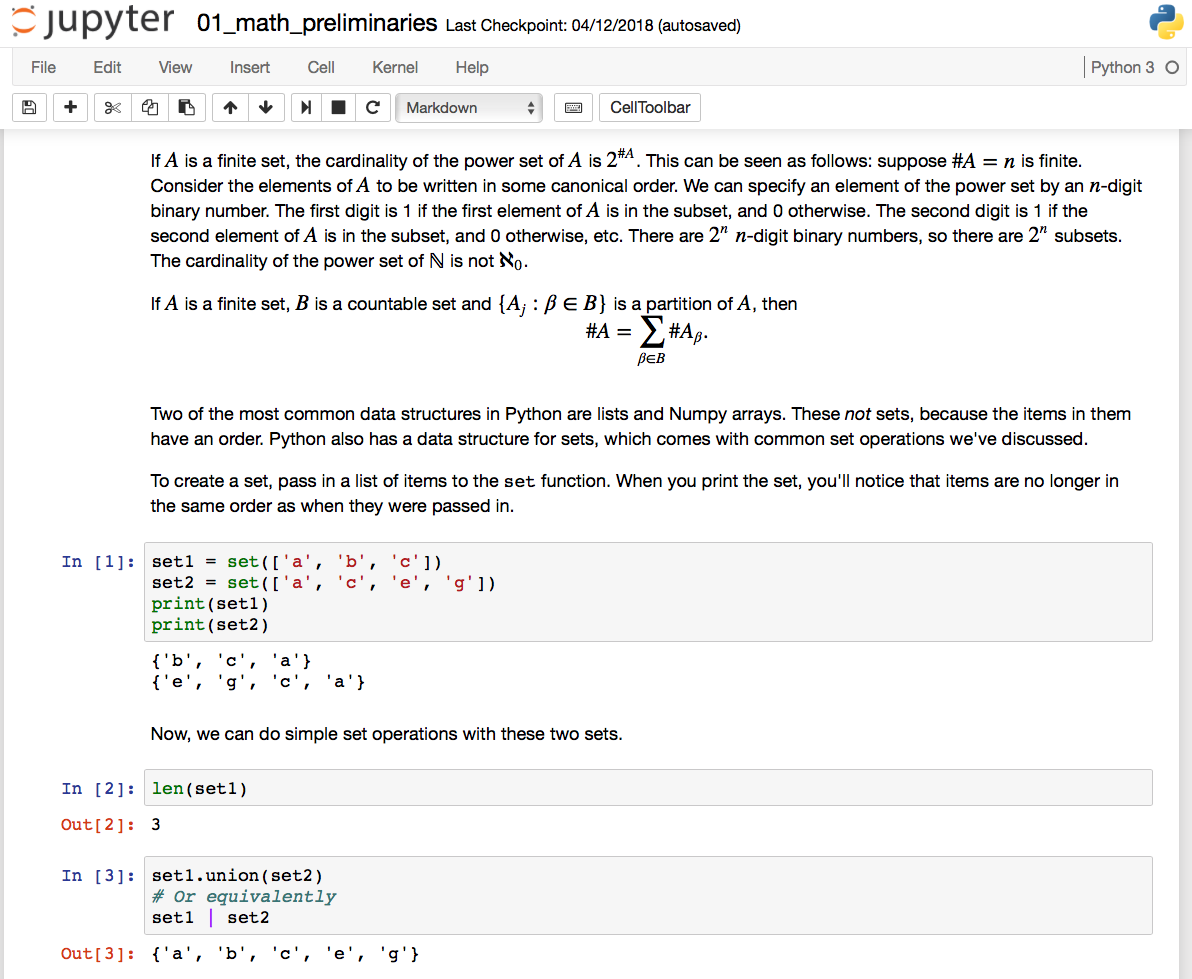
\includegraphics[height=0.8\paperheight]{fig/jupyter_notebook.png}};
  \node (img2) at (img1.east)[xshift=-1cm,yshift=-1.5cm] {
\includegraphics[height=0.15\paperheight]{fig/binder.png}};
\end{tikzpicture}
\end{center}

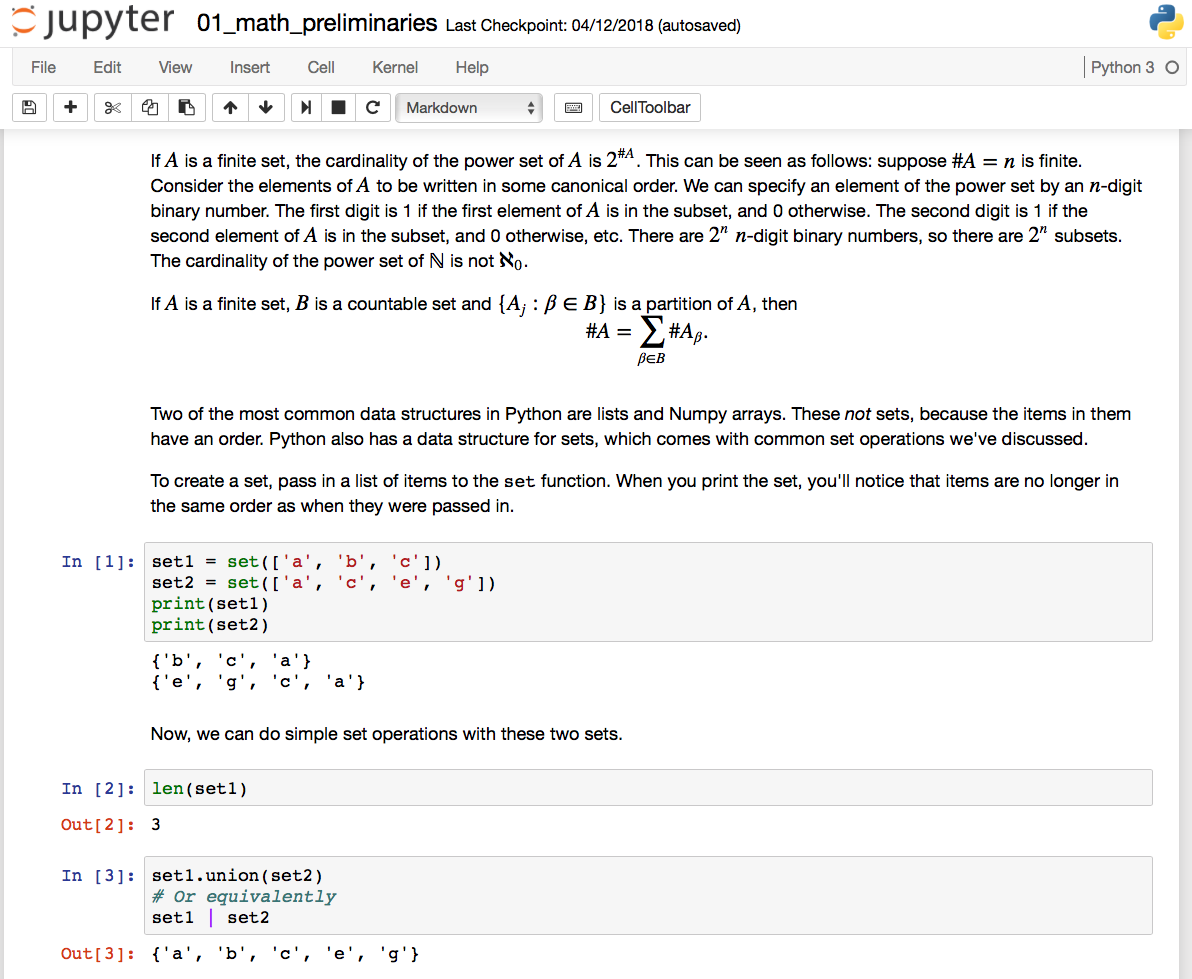
\includegraphics[height=\paperheight]{fig/jupyter_notebook.png}

\includegraphics{fig/binder.png}
}


\section[Components of a Permutation Test]{Components of a Permutation Test}

\usebackgroundtemplate{%             declare it
\tikz[overlay,remember picture] \node[opacity=0.3, at=(current page.center)] {
   
\includegraphics[height=\paperheight,width=1.2\paperwidth]{fig/clinical_trial.jpg}};
}


\frame{
\begin{center}
\Huge
Choosing a test statistic \\
\vspace{25pt}
Example: clinical trials
\end{center}
}

\usebackgroundtemplate{ }    %% undeclare it


\frame{
\frametitle{Clinical trial data}

Randomized experiment to treat GERD
\begin{itemize}
\item 136 patients
\item 8 sites
\item 7 clinical endpoints, baseline $X$ and follow-up $Y$ measures 
\end{itemize}

\vspace{10pt}
Did treatment A reduce symptoms compared to treatment B?

\begin{figure}
\centering
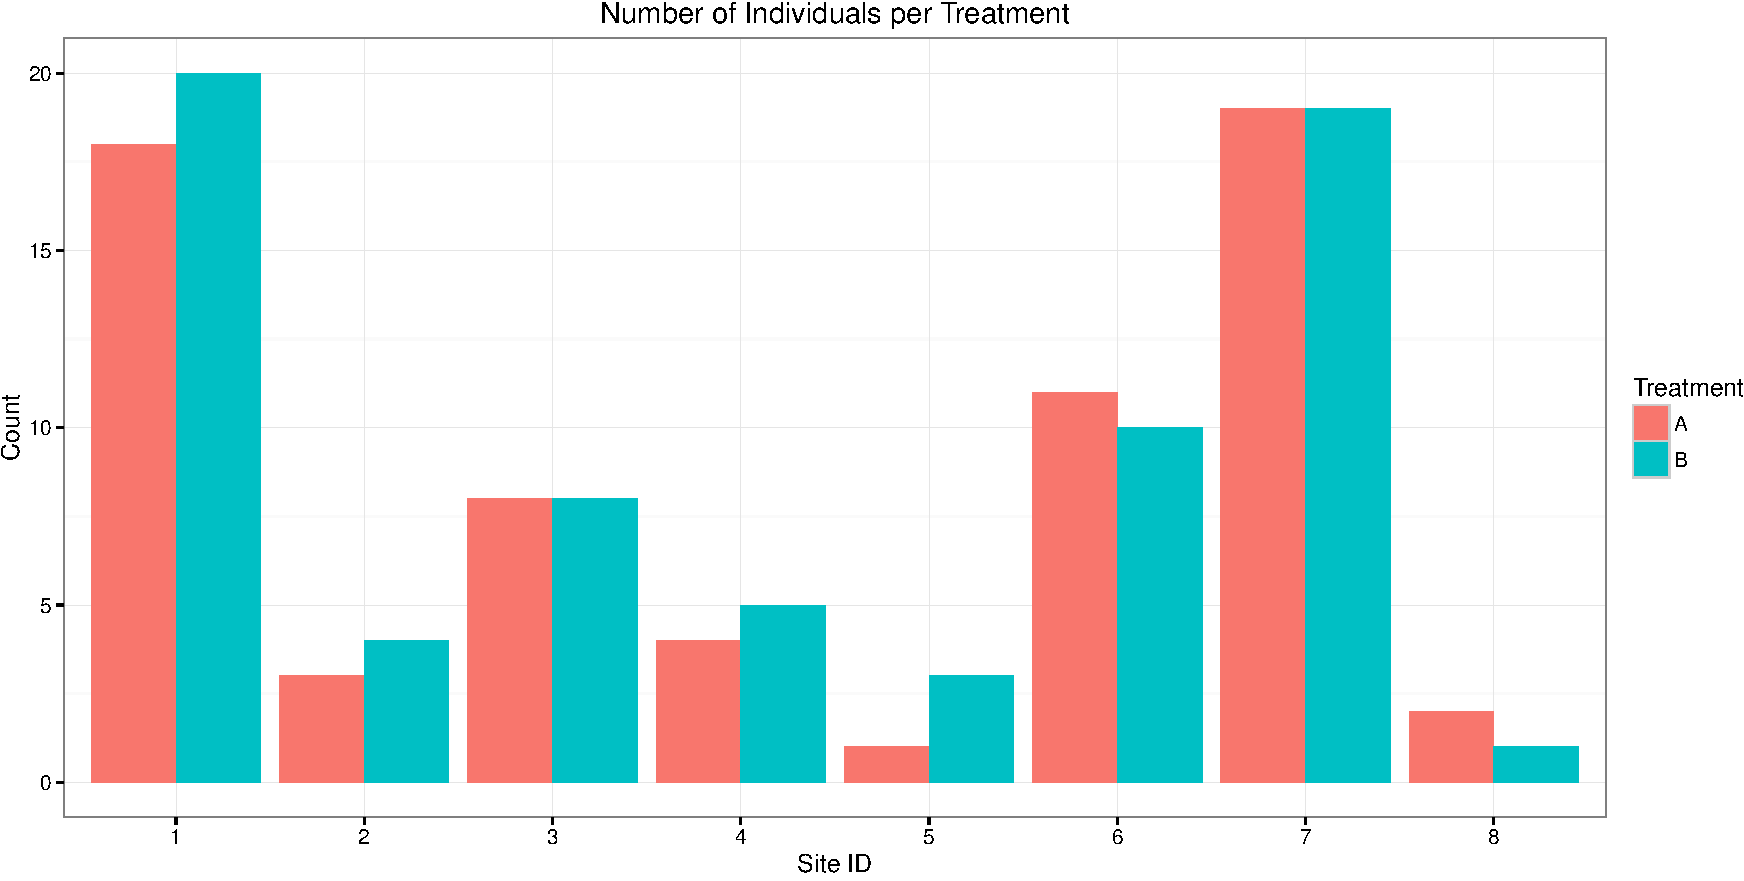
\includegraphics[width=0.7\textwidth]{fig/count_by_site-1.pdf}
\end{figure}


\vfill
\small \textit{Ottoboni, Lewis, and Salmaso (2018)}
}

\frame{
\frametitle{The permutation test}
Test the \textbf{sharp null hypothesis} that treatment has no effect:

$$H_0: Y_{ij}(A) = Y_{ij}(B), \forall \text{individuals }i \text{ and sites } j$$

\begin{figure}
\centering
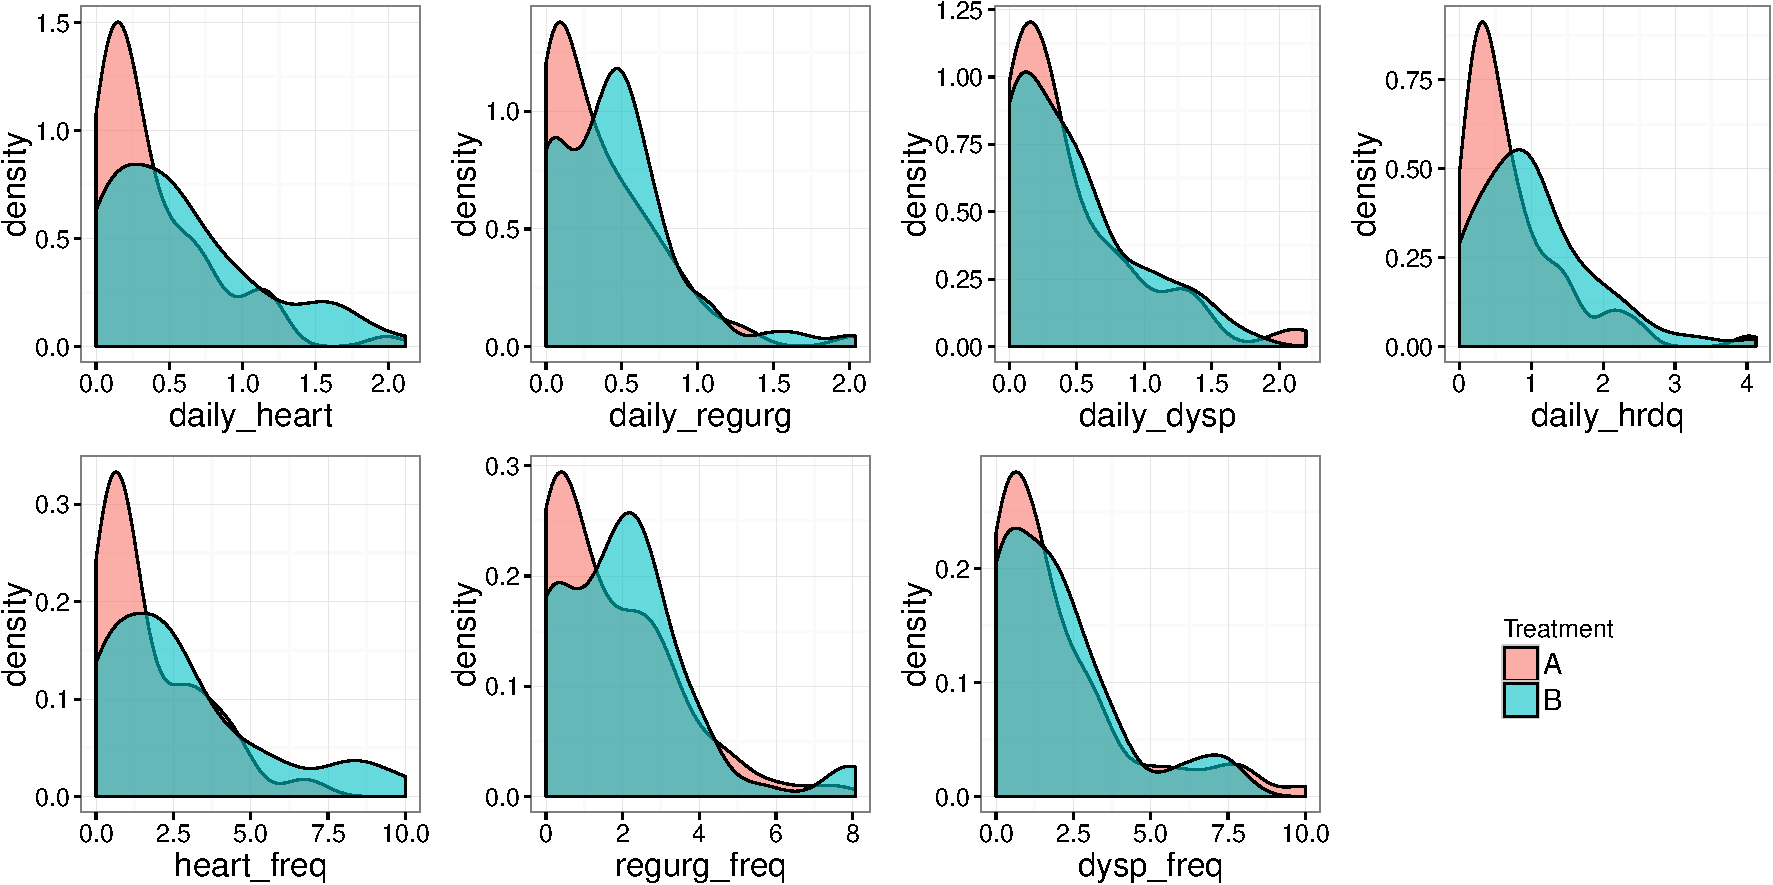
\includegraphics[width=0.7\textwidth]{fig/hist_continuous_vars-1.pdf}
\end{figure}

\vspace{5pt}

Naive, but correct, statistic: difference in mean outcomes
$$\overline{Y(A)} - \overline{Y(B)}$$


}

\frame{
\frametitle{Controlling for covariates}
\begin{itemize}
\itemsep 20pt
\item Difference scores: $\left( \overline{Y(A)} - \overline{X(A)} \right) - \left( \overline{Y(B)} - \overline{X(B)} \right)$
\item $t$ statistic from a linear model
$$ Y_{ij} = \alpha_j + \beta X_{ij} + \gamma Z_{ij} + \varepsilon_{ij}$$
\item Two ways to find a permutation distribution:
\begin{itemize}
\item Permute $Z$ 
\item Permute estimates $\hat{\varepsilon}$ from reduced model (\textit{Freedman and Lane (1983)})
\end{itemize}
\end{itemize}

}





\section[Randomized Experiments and Observational Studies]{Randomized Experiments and Observational Studies}

\usebackgroundtemplate{%             declare it
\tikz[overlay,remember picture] \node[opacity=0.3, at=(current page.center)] {
   \includegraphics[height=\paperheight,width=\paperwidth]{fig/set.jpg}};
}


\frame{
\begin{center}
\Huge
Randomized experiments \\
\vspace{25pt}
Example: student evaluations of teaching
\end{center}
}

\usebackgroundtemplate{ }    %% undeclare it



%\frame
%{
%  \frametitle{Teaching Evaluations}
% \begin{center}
% \Large{ Student evaluations of teachers (SET) are used to} \\
%  \begin{itemize}
%  \item Quantify teaching effectiveness
%  \item Compare instructors across courses
%  \item Make hiring, firing, and promotion decisions  
%  \end{itemize}
%  \vfill
%\end{center}
%}


\frame{
\frametitle{Teaching evaluations}
\large

Are SET a valid measure of teaching effectiveness? 
\vspace{15pt}

Data from MacNell et al. (2014)

\begin{center}
\begin{itemize}
\itemsep 10pt
\item Students were randomized to 4 online sections of a course.
\item In two sections, the instructors swapped identities.
\item Was the instructor who identified as female rated lower on average?
\end{itemize}
\end{center}

\vfill
\small \textit{Boring, Ottoboni, and Stark (2016)}
}


\frame{
\frametitle{Neyman-Rubin model, generalized}
%Student $i$ is represented by a ticket with $4$ numbers, their response to each ``treatment.''

\begin{align*}
\text{Rating } r_{ijk} &= \text{ SET given by student }i\text{ to instructor }j \\
&\text{ when they appear to have gender }k
\end{align*}
%$$i = 1, \dots, N; \qquad j = 1,2; \qquad k \in \{ \text{male, female} \}$$

\vspace{10pt}
%Numbers are fixed; randomization reveals one of the numbers. \\
%\vspace{10pt}
%Assume non-interference: each student's response depends only on that student's treatment. \\
\vspace{10pt}
If gender doesn't matter, $r_{ij\text{male}} = r_{ij\text{female}}.$

\vspace{20pt}
\begin{block}{Stratified two-sample test}
\begin{itemize}
\item For each instructor, permute perceived gender assignments
\item Use difference in mean ratings for female-identified minus male-identified
\end{itemize}
\end{block}
}



\frame
{
  \frametitle{Results}
In all categories, the male-identified instructor was rated higher.
\begin{table}
\begin{tabular}{r|crr}
\textbf{Characteristic} & \textbf{M-F} & \textbf{perm} $P$ & \textbf{t-test} $P$ \\
\hline
Overall & 0.47 & 0.12 & 0.128\\
Caring & 0.52 & 0.10 & 0.071\\
Consistent & 0.47 & 0.21 & \textcolor{red}{0.045} \\ 
Enthusiastic & 0.57 & 0.06 & 0.112 \\
Fair & 0.76 & \textcolor{red}{0.01} & 0.188 \\
Feedback & 0.47 & 0.16 & 0.054 \\
Helpful & 0.46 & 0.17 & \textcolor{red}{0.049} \\
Knowledgeable & 0.35 & 0.29 & \textcolor{red}{0.038} \\
Praise & 0.67 & \textcolor{red}{0.01} & 0.153 \\
Professional & 0.61 & 0.07 & 0.124 \\
Prompt & 0.80 & \textcolor{red}{0.01} & 0.191 \\
Respectful & 0.61 & 0.06 & 0.124 \\
Responsive & 0.22 & 0.48 & \textcolor{red}{0.013}
\end{tabular}
\end{table}

}






\section[Software and Statistics]{Algorithms and Pseudorandom Numbers}

\usebackgroundtemplate{%             declare it
\tikz[overlay,remember picture] \node[opacity=0.6, at=(current page.center)] {
   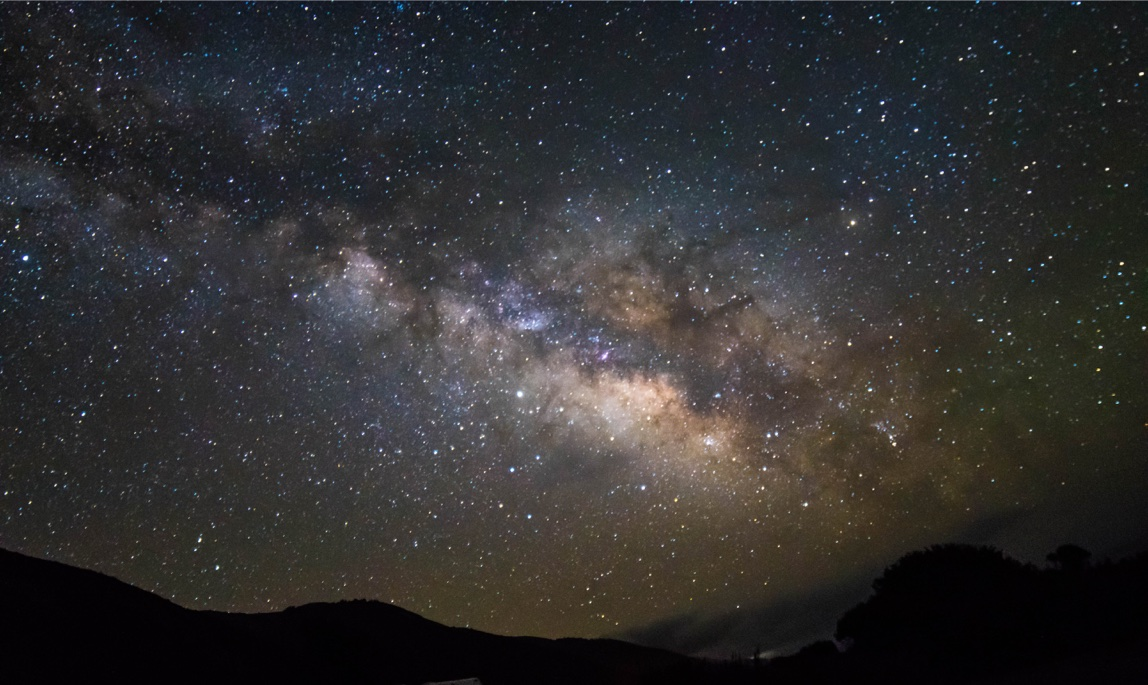
\includegraphics[height=\paperheight,width=\paperwidth]{fig/prngs.jpg}};
}


\frame{
\begin{center}
\Huge
Pseudorandom number generators
\end{center}
}

\usebackgroundtemplate{ }    %% undeclare it





\frame{
\frametitle{What is a PRNG?}

%A PRNG is a deterministic function with several components:
\begin{itemize}
\item A user-supplied \textbf{seed value} used to set the internal state
\item A function that maps the \textbf{internal state to pseudorandom bits}
\item A function that \textbf{updates the internal state}
\end{itemize}

\begin{center}
\resizebox{10cm}{!}{    
\begin{tikzpicture}[node distance = 3cm, auto, scale = 0.5]
    % Place nodes
    \node[io] (seed) {Seed};
    \node [f, right of=seed, node distance = 3cm] (state) {Internal state};
    \node [message, right of=state, node distance = 3cm] (output) {Random bits};
    % Draw edges
    \path [line] (seed) -- (state);
    \path [line] (state) -- (output);
    \path (state) edge [->, in = 130, out = 50, distance = 20mm] node[above] {Update} (state);
    % Draw box 
    \draw ($(state.north west)+(-2.5,2.5)$)  rectangle ($(state.south east)+(2.5,-1)$);
\end{tikzpicture}
}
\end{center}

}



\frame{
\frametitle{Pigeonhole principle in action}

\begin{theorem}[Too few pigeons]
If ${n \choose k}$ is greater than the size of a PRNG's state space, then the PRNG cannot possibly generate all samples of size $k$ from a population of $n$.
\end{theorem}


\begin{center}
\begin{table}[htdp]
\begin{tabular}{LLLL}
PRNG & \# Internal states & \# Possibilities & Proportion of attainable possibilities \\
\hline
32-bit linear congruential generators & 4 billion & Samples of 10 out of 50 items $\approx 10$ billion & $0.4$ \\
\hline
Mersenne Twister & $\approx 2 \times 10^{6010}$ & Permutations of $2084$ items $\approx 3 \times 10^{6013}$ & $0.0001$
\end{tabular}
\end{table}%
\end{center}

}


\frame{
\frametitle{Cryptographically secure PRNGs}
\textbf{Hash functions} take in a message $x$ of arbitrary length and return a value $h(x)$ of fixed size (e.g. 256 bits)


\begin{center}
\resizebox{10cm}{!}{    
\begin{tikzpicture}[node distance = 1cm, auto, scale = 0.5]
    % Place nodes
    \node[io] (IV) {IV};
    \node [f, right of=IV] (f1) {f};
    \node [f, right of=f1] (f2) {f};
    \node [f, right of=f2, node distance=3cm] (fn1) {f};
    \node [f, right of=fn1] (fend) {f};
    \node [f, right of=fend] (g) {g};
    \node [io, right of=g] (hx) {$h(x)$};
    \node [message, above of=f1] (m1) {$x_1$};
    \node [message, above of=f2] (m2) {$x_2$};
    \node [message, above of=fn1] (mn1) {$x_{n-1}$};
    \node [message, above of=fend] (mend) {$x_n$};
    \node [message, above right = of m1, above left = of mend, minimum width = 5cm] (message) {$x$};
    % Draw edges
    \path [line] (IV) -- (f1);
    \path [line] (f1) -- (f2);
    \path [line] (message) -- (m1);
    \path [line] (message) -- (m2);
    \path [line] (message) -- (mn1);
    \path [line] (message) -- (mend);
    \draw [-,dotted] (m2) -- (mn1);
    \path [line] (m1) -- (f1);
    \path [line] (m2) -- (f2);
     \path [line] (mn1) -- (fn1);
    \path [line] (mend) -- (fend);
    \path [line] (fend) -- (g);
    \path [line,dashed] (f2) -- (fn1);
    \path [line] (fn1) -- (fend);
    \path [line] (g) -- (hx);
\end{tikzpicture}
}
\end{center}
Cryptographic hash functions:
\begin{itemize}
\item computationally infeasible to invert
\item difficult to find two inputs that map to the same output
\item small input changes produce large, unpredictable changes to output
\item resulting bits are uniformly distributed
\end{itemize}
}

\frame{
\frametitle{From paper to program}
\Large

\begin{itemize}
\itemsep 15pt
\item Teach the concepts of hypothesis testing using permutation tests
\item Open-source online book with interactive Python examples
\item Packages on GitHub: \texttt{permute}, \texttt{cryptorandom}, \texttt{pscore\_match}
\end{itemize}

}


%\begin{frame}
%\frametitle{References}
%\tiny
%\bibliographystyle{plainnat}
%\bibliography{refs}
%\itemize
%\end{frame}


\end{document}
